% This the UCR_archive_wws--1/pgfplot_f1-score_wws=1.0.tex file.
% It was created by the python TexPlots class at 2021-10-16 13:33:42

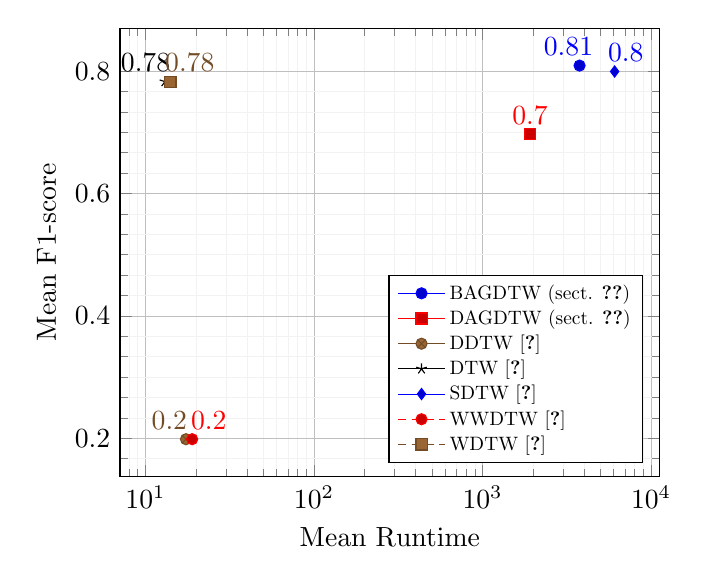
\begin{tikzpicture}
	\pgfplotstableread[col sep=comma]{%
		3764.188713644189, 0.8090116355217968
	}\bagdtw
	\pgfplotstableread[col sep=comma]{%
		1914.245479715869, 0.6970243067238234
	}\dagdtw
	\pgfplotstableread[col sep=comma]{%
		17.39747724943514, 0.19850928953229818
	}\ddtw
	\pgfplotstableread[col sep=comma]{%
		13.045470390868147, 0.7828110431764546
	}\dtw
	\pgfplotstableread[col sep=comma]{%
		6076.276831380926, 0.7993714863129143
	}\sdtw
	\pgfplotstableread[col sep=comma]{%
		18.933300181981483, 0.19850928953229818
	}\wddtw
	\pgfplotstableread[col sep=comma]{%
		14.06638409298067, 0.7828110431764546
	}\wdtw
	\begin{axis}[
		table/col sep = comma,
		xmode = log,
		xlabel = {Mean Runtime},
		ylabel = {Mean F1-score},
		grid = both,
		grid style={line width=.2pt, draw=gray!10},
		major grid style={line width=.2pt,draw=gray!50},
		minor tick num=5,
		legend cell align={left},
		legend pos = south east,
		legend style={nodes={scale=0.7, transform shape}},
		clip=false, % avoid clipping at edge of diagram
		nodes near coords, % print the value near node
	]
		\addplot+ [every node/.append style={xshift=-4pt}]  table[ x index = {0}, y index = {1}]{\bagdtw};
		\addplot+ [every node/.append style={xshift=0pt}]  table[ x index = {0}, y index = {1}]{\dagdtw};
		\addplot+ [every node/.append style={xshift=-6pt}]  table[ x index = {0}, y index = {1}]{\ddtw};
		\addplot+ [every node/.append style={xshift=-7pt}]  table[ x index = {0}, y index = {1}]{\dtw};
		\addplot+ [every node/.append style={xshift=4pt}]  table[ x index = {0}, y index = {1}]{\sdtw};
		\addplot+ [every node/.append style={xshift=6pt}]  table[ x index = {0}, y index = {1}]{\wddtw};
		\addplot+ [every node/.append style={xshift=7pt}]  table[ x index = {0}, y index = {1}]{\wdtw};
		\addlegendentry{BAGDTW (sect. \ref{sct:bagdtw})}
		\addlegendentry{DAGDTW (sect. \ref{sct:dagdtw})}
		\addlegendentry{DDTW \cite{keogh2001derivative}}
		\addlegendentry{DTW \cite{bellman1959adaptive}}
		\addlegendentry{SDTW \cite{cuturi2017soft}}
		\addlegendentry{WWDTW \cite{jeong2011weighted}}
		\addlegendentry{WDTW \cite{jeong2011weighted}}
	\end{axis}
\end{tikzpicture}
